\subsection{Resolved analysis results}
\label{sec:results}
%-------------------------------------------------------------------------------
%Table~\ref{tab:event_yields}  shows the number of events selected by
%the full analysis cut chain excluding the $m_{hh}$ cut.
%The observed data are in good agreement with the expected background  except for the
%\emph{high-mass} selection,  where a 20\% excess is found. Nevertheless, this  excess is
%not significant due to the  30\% systematic on the background
%prediction.
 
The resolved analysis  is described in detail in
Section~\ref{sec:Resolved}. The event selection is described in
Section~\ref{sec:resolved_selection} and summarized in
Table~\ref{tab:sig_reg_summary}. For each selected event, the
invariant mass of the $HH$ system ($m_{HH}$) is reconstructed and its distribution is shown in Figure~\ref{fig:mhh_1} for the \emph{non-res} and the \emph{m500} analyses, and in Figure~\ref{fig:mhh_2} for the \emph{low-mass} and the \emph{high-mass} analyses.
%After applying the requirements listed in Table \ref{tab:sig_reg_summary},  the invariant mass of the $HH$ system ($m_{HH}$) is distributed as shown in Figures \ref{fig:mhh_1} and \ref{fig:mhh_2}.
Data are generally in good agreement with the expected
background predictions within the total uncertainty.
The signal $m_{HH}$ distribution is shown in the figure for the non-resonant and the scalar resonance.
%At this selection stage, the non-resonant signal shows a broad
%distribution in $m_{hh}$ concentrated below 1 TeV.
Because the scalar-resonance samples are simulated in the narrow-width approximation,  the
reconstructed resonance width is exclusively due to the detector
resolution. 
%causes a sensitivity loss for the last signal model.
 
\begin{figure}
\begin{center}
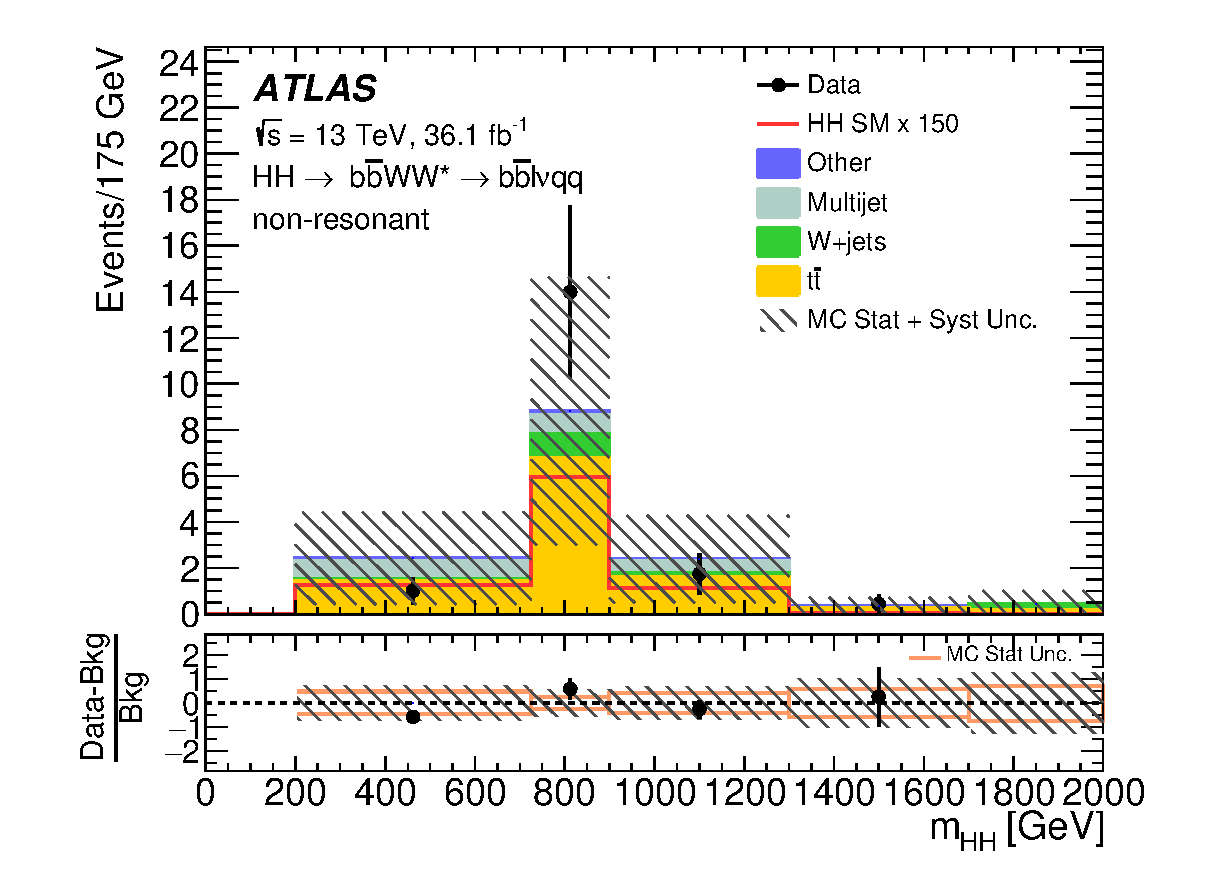
\includegraphics[width=0.75\textwidth]{paper_figures/C_reOptNonRes_mww_bbpt210_bbpt300_wwpt250_mbb_hhMass_regionA_met25d020}
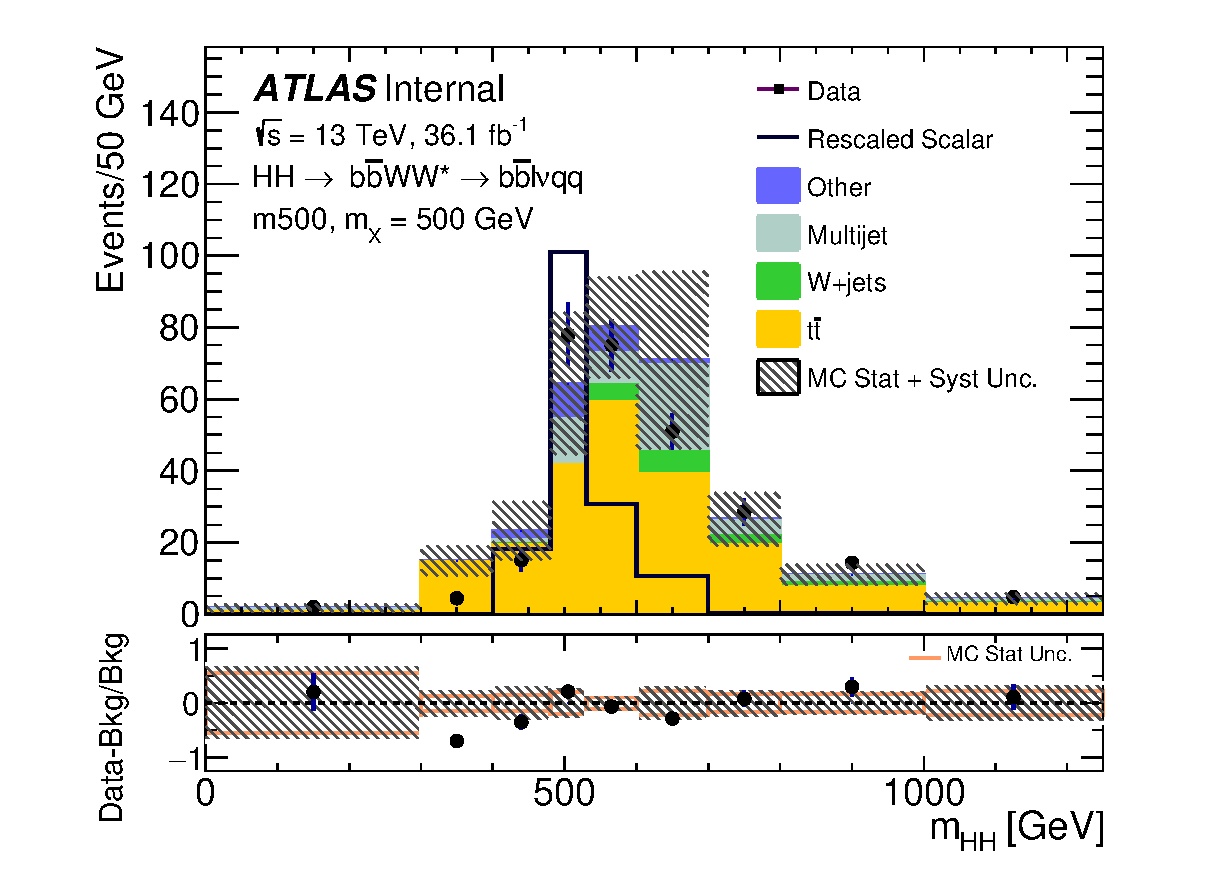
\includegraphics[width=0.75\textwidth]{paper_figures/C_reOpt500_mww_bbpt210_wwpt150_mbb_hhMass_regionA_met25d020}
\end{center}
\caption[$m_{HH}$ distributions for non-resonant and \emph{m500} selections in the resolved analysis]{$m_{HH}$ distributions for non-resonant and \emph{m500} selections in the resolved analysis. For each selection the corresponding signal hypothesis, non-resonant and scalar resonance, is shown. For the scalar signal, resonances with mass 500~\GeV\ are shown. The lower panel shows the fractional difference between data and the total expected background
 with the corresponding statistical and total uncertainty. The non-resonant signal is multiplied by a factor of 150 with respect to the expected SM cross section.  The scalar signal is multiplied by a factor of five with respect to the expected upper-limit cross section.)}%reported in Section~\ref{sec:Analysis_resil}. }
\label{fig:mhh_1}
\end{figure}
 
\begin{figure}
\begin{center}
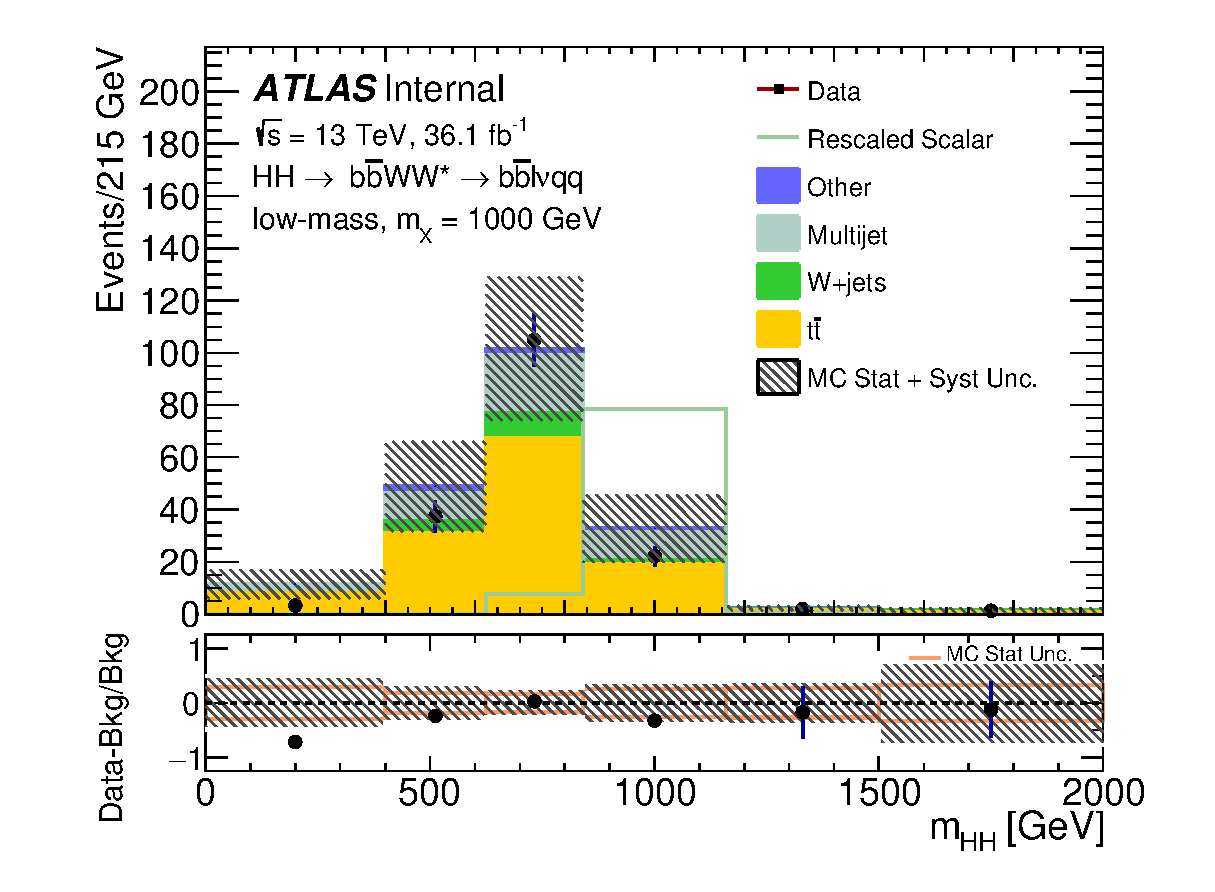
\includegraphics[width=0.75\textwidth]{paper_figures/C_reOpt700_mww_bbpt210_wwpt250_mbb_hhMass_regionA_met25d020}
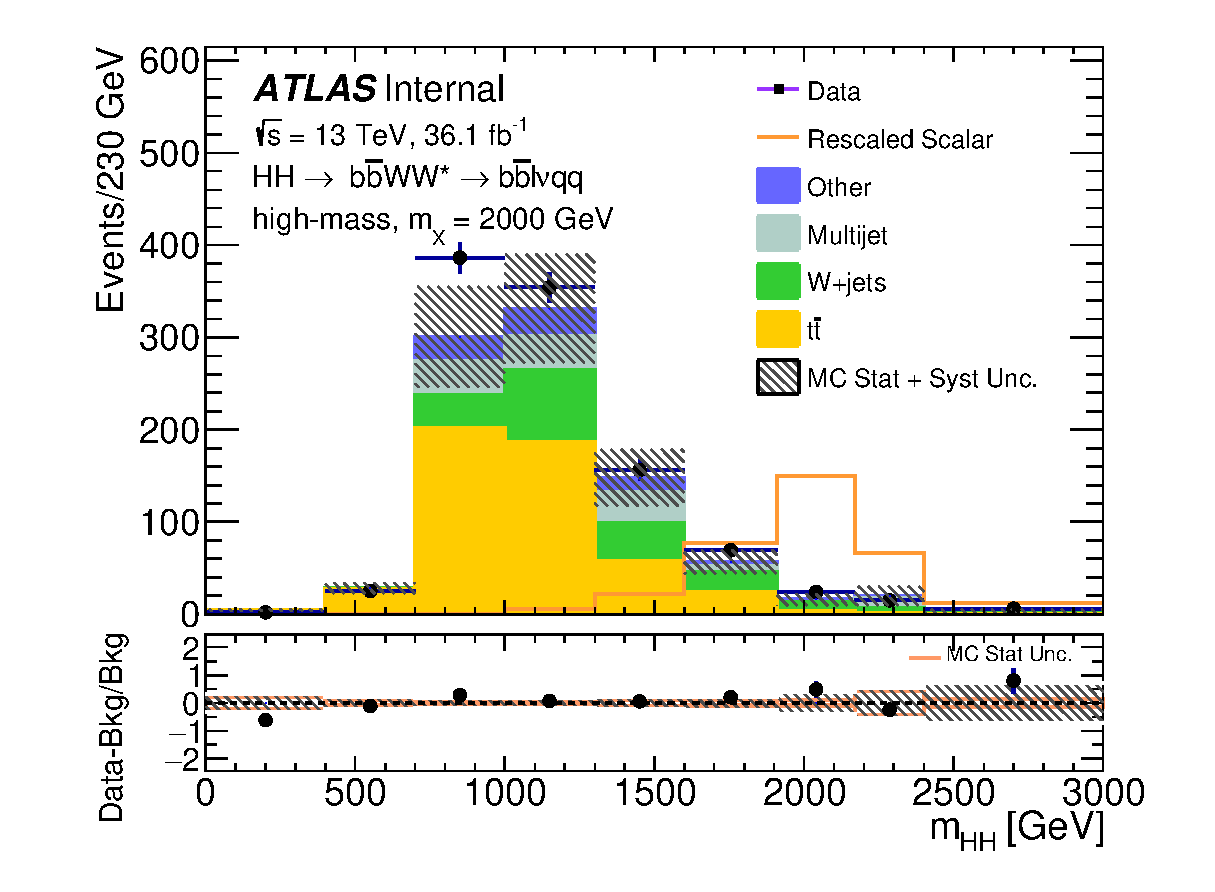
\includegraphics[width=0.75\textwidth]{paper_figures/C_reOpt2000_bbpt350_wwpt250_drww15_mbb_hhMass_regionA_met25d020}
\end{center}
\caption[$m_{HH}$ distributions for non-resonant and \emph{m500} selections in the resolved analysis for the low and high mass selections ]{$m_{HH}$ distributions in the resolved analysis selections. For each selection the corresponding
 signal hypothesis and mass 1000 (2000)~\GeV\ for the  \emph{low-mass} (\emph{high-mass}) analysis, are shown.  The lower panel shows the fractional difference between data and the total expected background
 with the corresponding statistical and total uncertainty. In the plot the scalar signal is multiplied by a factor of eight with respect to the expected upper-limit cross section;% reported in Section~\ref{sec:MainResults}; 
for the plot on the right
the multiplying factor is 20 for the scalar signal.}
\label{fig:mhh_2}
\end{figure}
 
 
The $m_{HH}$ distribution is sampled with resonance-mass-dependent
$m_{HH}$ requirements as reported in Table \ref{tab:mhh_sig_cuts}.
The numbers of events in the signal and control regions (the $t\bar{t}$
control region and the C region of the multijet estimation procedure) are
simultaneously fit using a  maximum-likelihood approach. The fit includes six contributions: signal, $W$+jets,
$Z$+jets, $t\bar{t}$, single-top-quark production, diboson and multijet. The
$t\bar{t}$ and multijet normalisations are free to float, the C
region of the ABCD method being directly used in the fit, while the
diboson, $W$+jets and $Z$+jets backgrounds are constrained
to the expected SM cross sections within their uncertainties.
 
The fit is performed after combining the electron and muon channel distributions. Statistical uncertainties due to the limited
sample sizes of the simulated background processes are taken into
account in the fit by means of nuisance parameters, which are
parameterised by Poisson priors. Systematic uncertainties are taken into account as
nuisance parameters with Gaussian constraints. For each
source of systematic uncertainty, the correlations across bins and
between different kinematic regions, as well as those between signal
and background, are taken into account.
Table~\ref{tab:event_yields_low} shows
the post-fit number of predicted backgrounds, observed data, and the
signal events normalized to the expected upper limit cross
sections. Expected event yields vary across mass because of varying selections. For instance, the requirement on $p_{\rm T}^{b \bar{b}}$ is higher in \emph{non-res} selection than in \emph{low-mass} selection. Similarly, even within \emph{low-mass} or \emph{high-mass} selection, the requirement on $m_{HH}$ vary across mass.  
 
 
\begin{table}
\small
\begin{center}
\begin{tabular}{r|*{4}{r@{}c@{}l|}r}
\hline
\multicolumn{14}{c}{Resonant analysis} \\
\hline
$m_X$ [GeV] & \multicolumn{3}{c}{$S$} & \multicolumn{3}{c}{Total Bkg.} & Data \\
\hline
500~~~~~~& 18  &$\,\pm\,$&5   & 19&$\,\pm\,$&6 & 26 \\
600~~~~~~& 13  &$\,\pm\,$&2   & 17&$\,\pm\,$&6 & 16 \\
700~~~~~~& 16  &$\,\pm\,$&2   & 25&$\,\pm\,$&8 & 22 \\
750~~~~~~& 20  &$\,\pm\,$&2   & 22&$\,\pm\,$&9 & 27 \\
800~~~~~~& 18.4&$\,\pm\,$&1.5 & 20&$\,\pm\,$&8 & 28 \\
900~~~~~~& 16.3&$\,\pm\,$&1.6 & 20&$\,\pm\,$&7 & 23 \\

1000~~~~~~& 12.0&$\,\pm\,$&1.3 & 14&$\,\pm\,$&5 & 11 \\
1100~~~~~~& ~~9.6&$\,\pm\,$&1.2 & ~~8&$\,\pm\,$&3 & 8\\
1200~~~~~~& ~~8.1&$\,\pm\,$&0.9 & ~~6&$\,\pm\,$&3 & 5 \\
1300~~~~~~& ~~5.1&$\,\pm\,$&0.7 & ~~3.5&$\,\pm\,$&1.8 & 1\\
1400~~~~~~& 4.3&$\,\pm\,$&0.3 &  ~~1.1&$\,\pm\,$&0.2 & 0 \\
1500~~~~~~& 3.5&$\,\pm\,$&0.3 & 1.1&$\,\pm\,$&0.2 & 0 \\
1600~~~~~~& 3.1&$\,\pm\,$&0.3 & ~~0.4&$\,\pm\,$&0.3 & 1 \\
1800~~~~~~& 14.1&$\,\pm\,$&1.8 & 17&$\,\pm\,$&5 & 21 \\
2000~~~~~~& 8.7&$\,\pm\,$&1.0 & 8&$\,\pm\,$&3 & 9 \\
2250~~~~~~& 7.9&$\,\pm\,$&1.1 & 6&$\,\pm\,$&2 & 7 \\
2500~~~~~~& 5.5&$\,\pm\,$&0.8 & 3.3&$\,\pm\,$&1.4 &  3\\
2750~~~~~~& 5.7&$\,\pm\,$&1.0 & 3.1&$\,\pm\,$&1.3 & 3\\
3000~~~~~~& 4.3&$\,\pm\,$&0.7 & 2.1&$\,\pm\,$&1.0 & 1 \\
\hline
\multicolumn{14}{c}{Non-resonant analysis} \\
\hline
\multicolumn{10}{c|}{Rescaled SM signal} & \multicolumn{3}{c}{Total Bkg.} & Data \\
\hline
\multicolumn{10}{c|}{17$\,\pm\,$2} & 21&$\,\pm\,$&8 & 22\\
\end{tabular}
\caption[Data event yields, and post-fit signal and background event yields in the final signal region for the non-resonant analysis and the resonant analysis]{Data event yields, and post-fit signal and background event yields in the final signal region for the non-resonant analysis and the resonant analysis in the 500--3000~\GeV\ mass range. The errors shown
are the MC statistical and systematic uncertainties described in
Section~\ref{sec:systematics}. The yields are shown for a scalar ($S$) signal model. Signal event yields are normalized to the expected upper-limit cross section.}  
\label{tab:event_yields_low}
\end{center}
\end{table}
 
 
No significant excess over the expectation is observed and the results are used to evaluate an upper limit at the $95\%$
confidence level (CL)  on the production cross section times the
branching fraction for the signal hypotheses under consideration.
The exclusion limits are calculated with a modified frequentist
method~\cite{CLs_2002}, also known as CL$_{\mathrm{s}}$, and the
profile-likelihood test statistic~\cite{asymptotics}.  None of the considered
systematic uncertainties is significantly constrained or
pulled in the likelihood fit.
 
In the SM signal hypothesis the observed (expected) upper
limit on the $\sigma(pp \to HH) \times {\mathcal{B}}( HH \to b\bar{b}WW^{\ast})$ at 95\%
CL is:
\[
\sigma(pp \to HH) \cdot {\mathcal{B}}(HH \to b\bar{b}WW^{\ast}) < 2.5 \, \left
 (2.5^{+1.0}_{-0.7} \right )  \,
{\mathrm{pb}}.
\]
The branching fraction ${\mathcal{B}}(HH \to b\bar{b}WW^{\ast}) = 2\times
{\mathcal{B}}(H \to b\bar{b}) \times {\mathcal{B}}(H \to WW^{\ast}) = 0.248$ is used to
obtain the following observed (expected) limit on the $HH$ production cross section at 95\% CL:
\[
\sigma(pp \to HH) < 10 \, \left (10^{+4}_{-3} \right) \,  {\text{pb,}}
\]
 
which corresponds to 300~(300$^{+100}_{-80}$) times the SM predicted cross section.
Including only the statistical uncertainty, the expected upper limit for the non-resonant production is
190 times the SM prediction.
This result, when compared with other $HH$ decay channels, is not competitive.  This is mainly  due to the similarity of the reconstructed $m_{HH}$ spectrum between the non-resonant SM signal
and the $t\bar{t}$ background that makes the separation between the
two processes difficult.
 
Figure~\ref{fig:limit} shows the expected and observed limit
curves for the production cross section of a scalar $S$ particle.
Different selections are used in different resonance mass ranges without attempting to statistically combine them. The
switch from one selection to another is performed based on the
best expected limit for that resonance mass.
The outcome of this procedure is that the \emph{m500} selection is used to set limits on resonances of mass of 500 GeV,  the \emph{low-mass}   selection is used up to masses of 1600 GeV, while the \emph{high-mass} selection is used in the mass range 1600-3000 GeV.
 
 
\begin{figure}[!h]
\begin{center}
\includegraphics*[width=0.95\textwidth]{paper_figures/limit_2016_reOpt_HiggsApproved_Scalar_Resolved_Paper_20180620_03.eps}
%\includegraphics*[width=0.45\textwidth]{paper_figures/limit_2016_reOpt_HiggsApproved_Grav_Paper_Resolved_20180920_00.eps}
\caption[Expected and observed upper limit at 95\% CL on the cross section of resonant pair
         production for the resolved analysis in the heavy scalar boson $S$ model]{Expected and observed upper limit at 95\% CL on the cross section of resonant pair
         production for the resolved analysis in the heavy scalar boson $S$ model. The plot also shows the expected limit
         without including the systematic errors in order to show their impact.
         %The impact of systematic errors is similar in
         %the scalar and the two graviton interpretation cases,
         %therefore the statistics only limit is not shown in the last
          %case for clarity.
          }
\label{fig:limit}
\end{center}
\end{figure}
 
 
Overall, the resolved analysis is most sensitive for a mass value of 1300~\GeV\ with an
expected upper limit of 0.35~pb on $\sigma(pp \to HH)$. At this mass the observed exclusion limit  is 0.2~pb.
%For the resonant hypothesis the expected and observed limits are
%shown in Figure~\ref{fig:limit}.
In both the non-resonant and resonant cases, the impact of the
systematic uncertainties is observed to be large.
In order to quantify the impact of the
systematic uncertainties, a fit is performed where the estimated
signal yield,  normalized to an arbitrary cross-section value, is multiplied
by a scaling factor $\alpha_{\mathrm{sig}}$, which is treated as
the parameter of interest in the fit.
The fit is performed using pseudo-data and the contribution to the  uncertainty in
$\alpha_{\mathrm{sig}}$ from several sources is determined. The contribution of the statistical uncertainty  to the total
uncertainty in $\alpha_{\mathrm{sig}}$, shown in Table~\ref{tab:pre-fit-stat},  is decomposed into
signal region statistics, top CR statistics and multijet CR
statistics. The contribution of the systematic uncertainties to the
total uncertainty is decomposed into the dominant components and shown in Table~\ref{tab:pre-fit-systematics}. The dominant
systematic uncertainties vary across the mass range, but some of the most relevant ones are due to $t \bar{t}$ modelling, $b$-tagging systematic uncertainties, and those related to jet measurements.
 
%%%%%%%%%
\begin{table}

\begin{center}
\begin{tabular}{l|c|c|c|c}
Statistical source & \multicolumn{4}{c}{Resolved analysis} \\
\hline
           & \emph{Non-Res} (\%) &  500~\GeV\ (\%)  & 1000~\GeV\ (\%) & 2000~\GeV\ (\%)\\
\hline
 % & \multicolumn{3}{c}{\emph{Non-Res} (\%)} &  \multicolumn{3}{c}{500~\GeV\ (\%)}  & \multicolumn{3}{c}{1000~\GeV\ (\%)} & \multicolumn{3}{c}{2000~\GeV\ (\%)} \\
Signal region     & +60/--40 & +60/--60 & +70/--60& +80/--70    \\
Top control region       & +40/--30 & +28/--30 & +20/--12 & +13/--13 \\
Multijet control region & +40/--30 & +24/--26 & +30/--30 & +30/--30\\
\hline
Total statistical & +80/--60 & +70/--70     & +80/--70 & +90/--80  \\
 
\end{tabular}
\caption[Statistical contribution (in percentage) to the total error
 in the scaling factor $\alpha_{\mathrm{sig}}$ for
 the non-resonant signal and three scalar-signal mass hypotheses, 500~\GeV, 1000~\GeV\ and 2000~\GeV,
 in the resolved analysis]{Statistical contribution (in percentage) to the total error
 in the scaling factor $\alpha_{\mathrm{sig}}$ for
 the non-resonant signal and three scalar-signal mass hypotheses, 500~\GeV, 1000~\GeV\ and 2000~\GeV,
 in the resolved analysis. The values are extracted by
 calculating the difference in quadrature between the total
 statistical error and the error obtained after setting constant the normalisation
 factor of the background that dominates the region of interest.}
  \label{tab:pre-fit-stat}
\end{center}
\end{table}
%%%%%%%%%%%%%%
 
\begin{table}
\begin{center}
\begin{tabular}{l*{4}{|r@{}c@{}l}}
Systematic source & \multicolumn{12}{c}{Resolved analysis} \\
\hline
 & \multicolumn{3}{c|}{\emph{Non-Res} (\%)} &  \multicolumn{3}{c|}{500~\GeV\ (\%)}  & \multicolumn{3}{c|}{1000~\GeV\ (\%)} & \multicolumn{3}{c}{2000~\GeV\ (\%)} \\
\hline
%$t\bar{t}$ normalisation     & +60/-40 & +40/-30 & +20/-6  & +30/-40
%& -  \\
%Multijet normalisation       & +30/-30 & +20/-20 & +50/-40 & +20/-30 \\
%$t\bar{t}$ CR multijet unc.  & +30/-20 & +30/-30 & +30/-20 & +6/-7  \\
$t\bar{t}$ modelling ISR/FSR & ~~~~+30&/&--20 &~~~~ +10&/&--5  &~~~~~  +7&/&--4  & ~~~~~+2&/&--2    \\
%$t\bar{t}$ CR multijet normalisation  & +30/-30 & +9/-4  & +10/-2 & +7/-6 \\
Multijet uncertainty         & +10&/&--10 & +20&/&--10  & +20&/&--20 & +30&/&--30 \\
$t\bar{t}$ Matrix Element                & +10&/&--10 & \multicolumn{3}{c|}{---}     & \multicolumn{3}{c|}{---}     & \multicolumn{3}{c}{---}     \\
$W+$jets modelling PDF       & +4&/&--7   & +10&/&--10 & +2&/&--6   & +7&/&--5  \\
$W+$jets modelling scale     & +9&/&--10  &  +9&/&--4  & +9&/&--2   & +20&/&--10 \\
$W+$jets modelling gen.    & +10&/&--8  & +10&/&--10 & +9&/&--1   & +9&/&--9  \\
$t\bar{t}$ modelling PS       & +3&/&--2   & +30&/&--20 & +20&/&--20 & +2&/&--2    \\
\hline
%$b$-tag light mistagging     & +30&/&--20 & +10&/&--4  & +6&/&--2   & +30&/&--30 \\
$b$ tagging    & +30&/&--20 & +11&/&--5  & +7&/&--6   & +30&/&--30 \\
 
%Jet energy scale             & +10&/&--20 & +20&/&--20 & +10&/&--8  & +10&/&--6  \\
JES/JER             & +13&/&--20 & +20&/&--20 & +50&/&--50  & +10&/&--6  \\
 
$E_\text{T}^\text{miss}$ soft term res.& +20&/&--20 & +8&/&--1   & +9&/&--7 &
                                                                     +7&/&--7 \\
Pile-up reweighting           & +3&/&--10 & +5&/&--3   & +9&/&--10  & +6&/&--6 \\
%$b$-tag charm mistagging     & +6&/&--5   & +10&/&--3  & +1&/&--6   & \multicolumn{3}{c|}{---}  \\
%Jet energy resolution        & +11&/&--2  & +4&/&--8   & +50&/&--50 & \multicolumn{3}{c|}{---} \\
\hline
Total systematic & +60&/&--80 & +70&/&--70     & +&60/&--70 & +40&/&--60  \\
\end{tabular}
\caption[Systematic contributions  (in percentage) to the total error in
 the scaling factor $\alpha_{\mathrm{sig}}$ for
 the non-resonant signal and three scalar-signal mass hypotheses, 500~\GeV, 1000~\GeV\ and 2000~\GeV,
 in the resolved analysis]{Systematic contributions  (in percentage) to the total error in
 the scaling factor $\alpha_{\mathrm{sig}}$ for
 the non-resonant signal and three scalar-signal mass hypotheses, 500~\GeV, 1000~\GeV\ and 2000~\GeV,
 in the resolved analysis. The first column quotes the source
of the systematic uncertainty. The $"-"$ symbol indicates that the specified source
is negligible. The contribution is obtained by calculating the
difference in quadrature between the total error in $\alpha_{\mathrm{sig}}$
and that obtained by setting constant the nuisance parameter(s)  relative to the
contribution(s) under study. }
\label{tab:pre-fit-systematics}
\end{center}
\end{table}
 
 
\clearpage

\subsection{Boosted analysis results}
\label{sec:boosted_results}
The boosted analysis applies the selection criteria described in
Section~\ref{sec:boosted_selection}. After applying the large-$R$ jet mass requirement
$90 < m_\text{Large-$R$ jet} < 140$~\GeV, the $m_{HH}$ distribution is
reconstructed and its shape is fit to data using MC
signal and background templates. The distribution is fit using 17
bins, with almost uniform width except at low and high $m_{HH}$, where
the bin width is modified in order to have a MC statistical uncertainty
%from the MC finite sample-size
smaller than 20\%. All backgrounds, except multijet, are
simulated using MC generators and normalized using the cross section of the
simulated process. The multijet background is estimated using the ABCD
method, and its normalisation obtained from this method is kept fixed in the fit. The bias due
to possible signal contamination in the ABCD regions was studied
and found to have negligible effect on the result.  The integral of the $m_{HH}$
distribution for the boosted analysis is shown in
Table~\ref{tab:event_yields_high}.
\begin{table}
\caption[Data event yields, and post-fit signal and background event yields in the final signal region for the boosted analysis and the scalar $S$ particle hypothesis]{Data event yields, and post-fit signal and background event yields in the final signal region for the boosted analysis and the scalar $S$ particle hypothesis. The errors shown are the MC statistical and systematic uncertainties described in Section~\ref{sec:boosted_systematics}. For illustration a signal mass point of
2000~\GeV\ is reported in the table. The signal samples are normalized to the expected upper limit cross sections.}  
\label{tab:event_yields_high}
\small
\begin{center}
\begin{tabular}{c|c|c|c|c|c}
$m_X$ [\GeV] & $S$ & $G^{\ast}_{\rm KK}$ ($c=1.0$) & $G^{\ast}_{\rm KK}$ ($c=2.0$) & Total Bkg. & Data
\vspace{0.2mm}\\
\hline
2000 & 28 $\pm$ 0.5  & 36.4 $\pm$ 0.8 & 43.0 $\pm$ 0.7   & 1255 $\pm$ 27  & 1107 \\
\end{tabular}
\end{center}
\end{table}
 
%The statistical analysis is conducted by combining the electron and muon channels into a single combined
%lepton channel.
Systematic uncertainties affecting the $m_{HH}$ shape are parameterised as linear functions of $m_{HH}$,
and the function parameters are treated as nuisance parameters in the fit. Statistical uncertainties due to the limited
sample sizes of the simulated background processes are taken into
account in the fit by means of further nuisance parameters, which are
parameterised by Poisson priors.
%In particular, one nuisance parameter is assigned to each bin in the $m_{HH}$ distribution.
 
The systematic uncertainties included in the fit are described in
Section~\ref{sec:boosted_systematics}. The contribution of the systematic uncertainties to the
total uncertainty is decomposed into the dominant components and summarized  in
Table~\ref{tab:boosed_nplist_systematics}. The most relevant
systematic uncertainties are due to the limited size of the MC
samples, the $t \bar{t}$ modelling and the $b$-tagging systematic uncertainties.
 
\begin{table}

\begin{center}
\begin{tabular}{l*{4}{|r@{}c@{}l}}
Uncertainty source & \multicolumn{12}{c}{Boosted analysis} \\
\hline
      & \multicolumn{3}{c|}{1500~\GeV\ [\%]} &  \multicolumn{3}{c|}{2000~\GeV\ [\%]}  & \multicolumn{3}{c|}{2500~\GeV\ [\%]} & \multicolumn{3}{c}{3000~\GeV\ [\%]} \\
\hline
Data statistics  & ~~+50&/&--52 & ~~+59&/&--61  &  ~~+64&/&--66  & ~~+70&/&--72    \\
Total systematic  & +87&/&--85 & +81&/&--79  &  +76&/&--75  & +71&/&--69    \\
\hline
\hline
MC statistics  & +42&/&--48 & +42&/&--50  &  +39&/&--48  & +39&/&--49    \\
$t\bar{t}$ modelling  & +29&/&--31 & +36&/&--38  &  +40&/&--45  & +32&/&--39    \\
Multijet uncertainty         & +11&/&--14 & +19&/&--23  & +16&/&--20 & +11&/&--16 \\
$W+$jets modelling       & +27&/&--30   & +8&/&--12 & +11&/&--10   & +11&/&--10  \\
Single-top modelling       & +22&/&--26   & +5&/&--6 & +4&/&--5   & +5&/&--5  \\
\hline
$b$ tagging     & +31&/&--19 & +36&/&--22  & +36&/&--17  & +34&/&--14 \\
JES/JER            & +14&/&--14 & +6&/&--6 & +14&/&--11  & +7&/&--9  \\
Large-$R$ jet         & +29&/&--10 & +27&/&--8 & +27&/&--7  & +29&/&--8  \\
\end{tabular}
\caption[Statistical and systematic contributions (in percentage) to
 the total error in the scaling factor $\alpha_{\mathrm{sig}}$ in the boosted analysis
 for four mass hypotheses: 1500~\GeV, 2000~\GeV, 2500~\GeV\ and 3000~\GeV]{Statistical and systematic contributions (in percentage) to
 the total error in the scaling factor $\alpha_{\mathrm{sig}}$ in the boosted analysis
 for four mass hypotheses: 1500~\GeV, 2000~\GeV, 2500~\GeV\ and 3000~\GeV.
 The first column quotes the source of the uncertainty.
 The contribution is obtained by calculating the
difference in quadrature between the total error in $\alpha_{\mathrm{sig}}$
and that obtained by setting constant the nuisance parameter(s)  relative to the
contribution(s) under study.
%The fit region that is mainly affected by the systematic
 % uncertainty is shown, together its fractional contribution to the
 % quoted uncertainty.
}
   \label{tab:boosed_nplist_systematics}
\end{center}
\end{table}




\renewcommand{\arraystretch}{1.5}
\begin{table}
\begin{center}
\begin{tabular}{l|c|c|c}
Sample        &    Yield &  Stats Err &   Systs Err \\
\hline
$t\bar{t}$    &  648.7   & $\pm$ 16.4    & $^{+177.3(+27.3\%)}_{-169.2(-26.1\%)}$ \\
W+Jets        &  217.0   & $\pm$ 6.5     & $^{+104.3(+48.1\%)}_{-100.9(-46.5\%)}$ \\
QCD           &  235.2   & $\pm$ 18.9    & $^{+181.8(+77.3\%)}_{-181.8(-77.3\%)}$ \\
Single-top    &  109.2   & $\pm$ 6.0     & $^{+86.0(+78.8\%)}_{-85.8(-78.6\%)}$ \\
Z+Jets        &  20.5    & $\pm$ 1.1     & $^{+11.2(+54.6\%)}_{-10.9(-52.9\%)}$ \\
Dibosons      &  24.4    & $\pm$ 1.9     & $^{+15.3(+62.6\%)}_{-14.7(-60.1\%)}$ \\
\hline
Prediction    &  1255.0  & $\pm$ 26.7    & $^{+324.3(+25.8\%)}_{-311.3(-24.8\%)}$ \\
Data          &  1107    & - & - \\
\hline
Data/Pred     &  0.88    & - & - \\
\hline
\end{tabular}
\end{center}
\caption[Predicted and observed yields in the signal region]{Predicted and observed yields in the signal region. Detector modeling
uncertainties, MC background modeling uncertainties are considered for the systematic uncertainties.
The expected background yields are predicted from MC and no normalization factors are applied.}
\label{tab:boosted_results_sr_yields}
\end{table}
\renewcommand{\arraystretch}{1.0}
\FloatBarrier

Figure~\ref{fig:boosted_postfit_mhh} shows the $m_{HH}$ distribution for
data and the background components for the boosted analysis.
Data are generally in good agreement with the background expectations within the quoted systematic errors.
The signal $m_{HH}$ distribution is shown in the figure for  the scalar resonance.
Figure~\ref{fig:boosted_only_limits} shows the observed and the expected
upper limit on the production cross section of the scalar $S$ particle.
\iffalse
The expected
sensitivity of the boosted analysis is better than the resolved one
for the mass of the resonance X ($X = S$)  $m_X> 1300$~\GeV\.
\fi
\begin{figure}
\begin{center}
%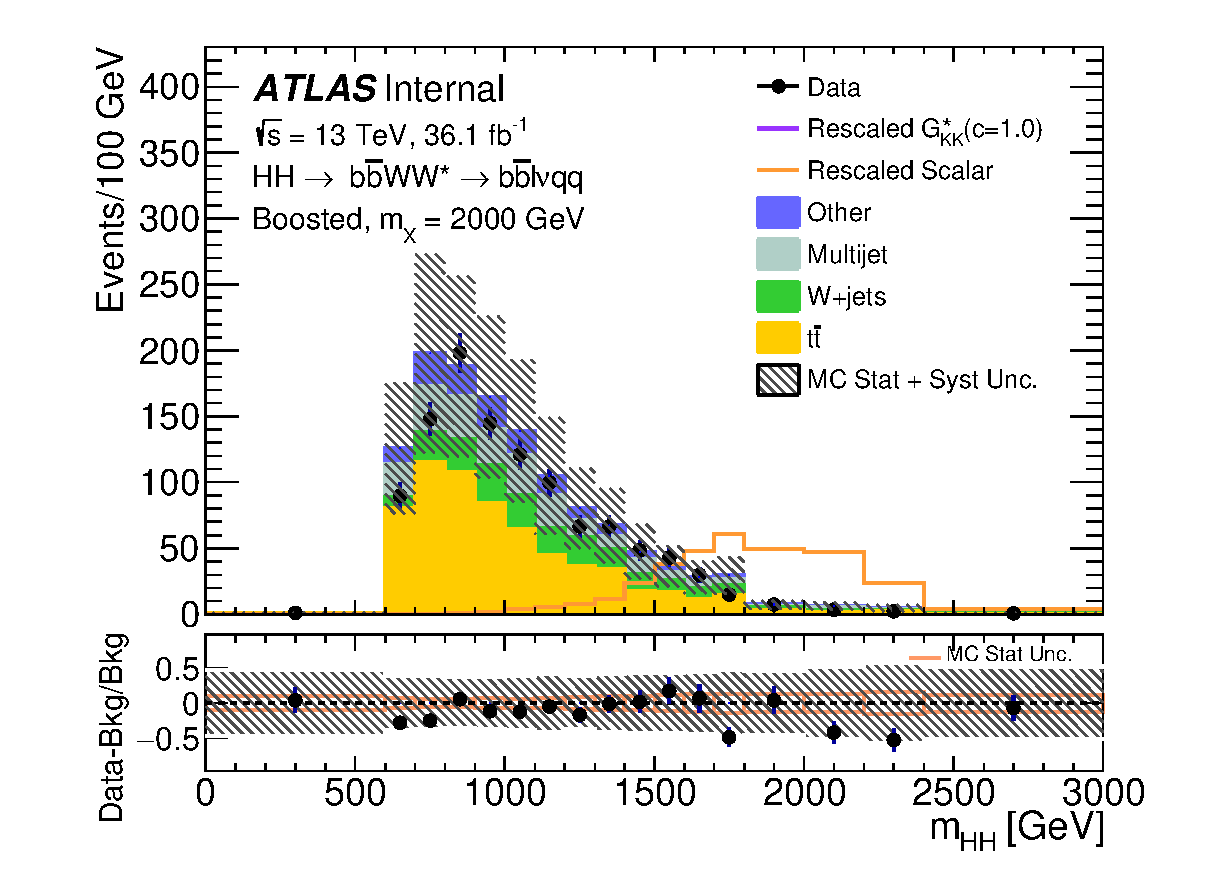
\includegraphics[height=0.55\textwidth]{figures/C_2tab_0bjet_SR_lepton_presel_met50_hhMassRebin1}
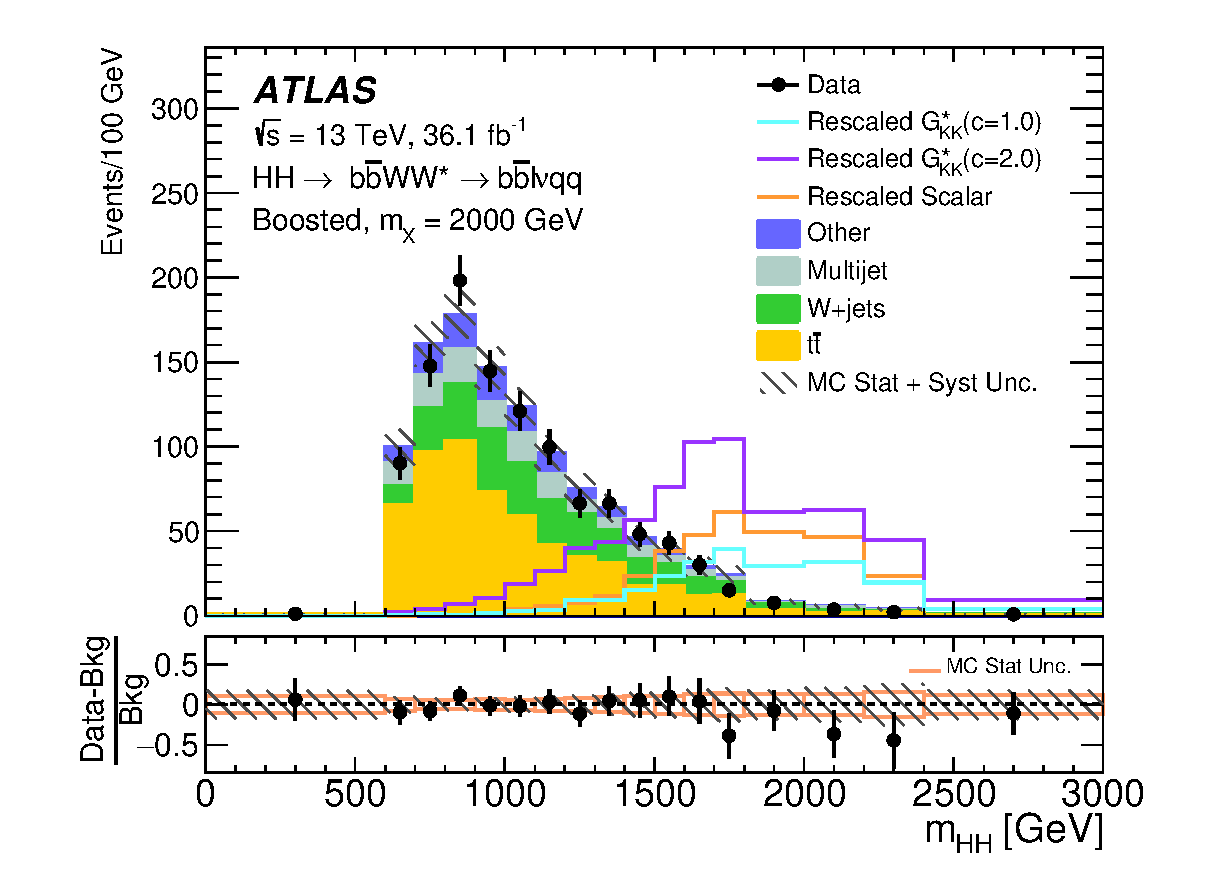
\includegraphics[width=0.95\textwidth]{paper_figures/C_2tab_0bjet_SR_lepton_presel_met50_hhMassRebin1_postfit.eps}
%\includegraphics[width=0.95\textwidth]{paper_figures/C_2tab_0bjet_SR_lepton_presel_met50_hhMassRebin1_2.eps} Prefit without Gkk

\end{center}
\caption[$m_{HH}$ distributions after the global likelihood fit for the boosted analysis]{$m_{HH}$ distributions after the global likelihood fit for the boosted analysis. The lower panel shows the fractional difference between data and the total expected background with the corresponding statistical and total uncertainty.  The signals shown correspond to resonances of mass 2000~\gev. The scalar signal is multiplied by a factor of four with respect to the expected upper-limit cross section.}%reported in Section~\ref{sec:MainResults}.}
  \label{fig:boosted_postfit_mhh}
\end{figure}
\FloatBarrier
 
\begin{figure}[!h]
\begin{center}
\includegraphics*[width=0.95\textwidth]{paper_figures/limit_2016_reOpt_HiggsApproved_Scalar_Boosted_Paper_20180620_00}
\caption[Expected and observed upper limits at 95\% CL on the cross section of resonant pair production for the heavy scalar boson $S$ model in the boosted analysis]{Expected and observed upper limits at 95\% CL on the cross section of resonant pair production for the heavy scalar boson $S$ model in the boosted analysis. The plot also shows the expected limits without including the systematic errors in order to show their impact.
         %The impact of systematic errors is similar in
         %the scalar and the two graviton interpretation cases,
         %therefore the statistics only limit is not shown in the last
          %case for clarity.
          }
 
\label{fig:boosted_only_limits}
\end{center}
\end{figure}
\subsection{Combined results}
Results of the two analyses are summarized in Figure~\ref{fig:combined_scalar_limit} for the scalar interpretation.
The sensitivity of the boosted analysis is higher than the resolved
analysis (the expected limit being lower)  for masses larger  than 1300 GeV in the scalar interpretation.
For masses lower than these values, the limits of the resolved analysis are presented in the figure, otherwise the boosted-analysis limits are shown.
In addition, the expected limits of both analyses are shown near the mass values where the switch between the two limit curves occurs.

Finally, the observed upper limits on the production cross sections range from 5.6~pb  for $m_X=500$~\GeV\ to 0.51~pb for
$m_X=3000$~\GeV\ for the scalar signal model. No boosted analysis was
performed for the non-resonant SM signal model.
 
For the non-resonant signal hypothesis the observed (expected) upper
limit on the $\sigma(pp \to HH) \times {\mathcal{B}}(HH \to b\bar{b}WW^{\ast})$ at 95\%
CL is:
\[
\sigma(pp \to HH) \cdot {\mathcal{B}}(HH \to b\bar{b}WW^{\ast}) < 2.5 \, \left
 (2.5^{+1.0}_{-0.7} \right )  \,
{\mathrm{pb}},
\]
which corresponds to 300~(300$^{+100}_{-80}$) times the SM predicted cross section.
\begin{figure}[!h]
\begin{center}
\includegraphics[height=0.95\textwidth]{figures/paper_figures/limit_2016_reOpt_HiggsApproved_Scalar_Paper_Combined_20190312_01}
\end{center}
\caption[Expected and observed cross section upper limit for the combines analysis]{Expected and observed upper limits at 95\% CL  on the cross-section of the resonant scalar signal model hypotheses. The observed limits of the scalar signal models are switched at a mass of 1300 GeV. The expected limits of both analyses are shown in a region around the switching points.
The switching point is chosen at the mass value where the boosted analysis becomes more sensitive than the resolved analysis. }
\label{fig:combined_scalar_limit}
\end{figure}
\FloatBarrier
 